%%
%% This is file `sample-sigconf.tex',
%% generated with the docstrip utility.
%%
%% The original source files were:
%%
%% samples.dtx  (with options: `sigconf')
%% 
%% IMPORTANT NOTICE:
%% 
%% For the copyright see the source file.
%% 
%% Any modified versions of this file must be renamed
%% with new filenames distinct from sample-sigconf.tex.
%% 
%% For distribution of the original source see the terms
%% for copying and modification in the file samples.dtx.
%% 
%% This generated file may be distributed as long as the
%% original source files, as listed above, are part of the
%% same distribution. (The sources need not necessarily be
%% in the same archive or directory.)
%%
%%
%% Commands for TeXCount
%TC:macro \cite [option:text,text]
%TC:macro \citep [option:text,text]
%TC:macro \citet [option:text,text]
%TC:envir table 0 1
%TC:envir table* 0 1
%TC:envir tabular [ignore] word
%TC:envir displaymath 0 word
%TC:envir math 0 word
%TC:envir comment 0 0
%%
%%
%% The first command in your LaTeX source must be the \documentclass
%% command.
%%
%% For submission and review of your manuscript please change the
%% command to \documentclass[manuscript, screen, review]{acmart}.
%%
%% When submitting camera ready or to TAPS, please change the command
%% to \documentclass[sigconf]{acmart} or whichever template is required
%% for your publication.
%%
%%
\documentclass[sigconf]{acmart}

%%
%% \BibTeX command to typeset BibTeX logo in the docs
\AtBeginDocument{%
  \providecommand\BibTeX{{%
    Bib\TeX}}}

%% Rights management information.  This information is sent to you
%% when you complete the rights form.  These commands have SAMPLE
%% values in them; it is your responsibility as an author to replace
%% the commands and values with those provided to you when you
%% complete the rights form.
\setcopyright{acmcopyright}
\copyrightyear{2018}
\acmYear{2018}
\acmDOI{XXXXXXX.XXXXXXX}

%% These commands are for a PROCEEDINGS abstract or paper.
\acmConference[Conference acronym 'XX]{Make sure to enter the correct
  conference title from your rights confirmation emai}{June 03--05,
  2018}{Woodstock, NY}
%%
%%  Uncomment \acmBooktitle if the title of the proceedings is different
%%  from ``Proceedings of ...''!
%%
%%\acmBooktitle{Woodstock '18: ACM Symposium on Neural Gaze Detection,
%%  June 03--05, 2018, Woodstock, NY}
\acmPrice{15.00}
\acmISBN{978-1-4503-XXXX-X/18/06}


%%
%% Submission ID.
%% Use this when submitting an article to a sponsored event. You'll
%% receive a unique submission ID from the organizers
%% of the event, and this ID should be used as the parameter to this command.
%%\acmSubmissionID{123-A56-BU3}

%%
%% For managing citations, it is recommended to use bibliography
%% files in BibTeX format.
%%
%% You can then either use BibTeX with the ACM-Reference-Format style,
%% or BibLaTeX with the acmnumeric or acmauthoryear sytles, that include
%% support for advanced citation of software artefact from the
%% biblatex-software package, also separately available on CTAN.
%%
%% Look at the sample-*-biblatex.tex files for templates showcasing
%% the biblatex styles.
%%

%%
%% The majority of ACM publications use numbered citations and
%% references.  The command \citestyle{authoryear} switches to the
%% "author year" style.
%%
%% If you are preparing content for an event
%% sponsored by ACM SIGGRAPH, you must use the "author year" style of
%% citations and references.
%% Uncommenting
%% the next command will enable that style.
%%\citestyle{acmauthoryear}


%%
%% end of the preamble, start of the body of the document source.
\begin{document}

%%
%% The "title" command has an optional parameter,
%% allowing the author to define a "short title" to be used in page headers.
\title{Ideas from the Synthesis Kernel in Modern Systems: Optimization techniques and SuperOptimizers}

%%
%% The "author" command and its associated commands are used to define
%% the authors and their affiliations.
%% Of note is the shared affiliation of the first two authors, and the
%% "authornote" and "authornotemark" commands
%% used to denote shared contribution to the research.
\author{Sridhara Madhu Mohan Nelemane}
\affiliation{%
 \institution{University of Bamberg}
 \city{Bamberg}
 \country{Germany}}

%%
%% By default, the full list of authors will be used in the page
%% headers. Often, this list is too long, and will overlap
%% other information printed in the page headers. This command allows
%% the author to define a more concise list
%% of authors' names for this purpose.
\renewcommand{\shortauthors}{Trovato et al.}

%%
%% The abstract is a short summary of the work to be presented in the
%% article.
\begin{abstract}

    The paper from Henry Massalin \cite{synthesis92} was considered futuristic 
    for its time. Several ideas were proposed in this paper towards developing
    a much more sophisticated operating system. These ideas particularly focussed 
    on performance of the operating system and an implementation called Synthesis
    kernel was used to drive the concept home. This seminar paper refers to the 
    same research and implementation and tries to provide an understanding
    some of the same ideas in the modern context. In particular the paper focuses on
    techniques of SuperOptimization utilized in Runtime Code Generation phase
    of the Synthesis Operating system. 

\end{abstract}

%%
%% The code below is generated by the tool at http://dl.acm.org/ccs.cfm.
%% Please copy and paste the code instead of the example below.
%%
\begin{CCSXML}
<ccs2012>
 <concept>
  <concept_id>10010520.10010553.10010562</concept_id>
  <concept_desc>Operating Systems Design</concept_desc>
  <concept_significance>500</concept_significance>
 </concept>
 <concept>
  <concept_id>10010520.10010575.10010755</concept_id>
  <concept_desc>Optimization</concept_desc>
  <concept_significance>300</concept_significance>
 </concept>
 <concept>
  <concept_id>10010520.10010553.10010554</concept_id>
  <concept_desc>SuperOptimization</concept_desc>
  <concept_significance>100</concept_significance>
 </concept>
 <concept>
  <concept_id>10003033.10003083.10003095</concept_id>
  <concept_desc>Synthesis Kernel</concept_desc>
  <concept_significance>100</concept_significance>
 </concept>
 <concept>
  <concept_id>10003033.10003083.10003095</concept_id>
  <concept_desc>Runtime Code Generation</concept_desc>
  <concept_significance>100</concept_significance>
 </concept>
</ccs2012>
\end{CCSXML}

\ccsdesc{Operating Systems Design-Performance}
\ccsdesc{Optimization - Techniques}
\ccsdesc{SuperOptimization}
\ccsdesc{Synthesis Kernel}
\ccsdesc{Runtime Code Generation}

%%
%% Keywords. The author(s) should pick words that accurately describe
%% the work being presented. Separate the keywords with commas.
\keywords{datasets, neural networks, gaze detection, text tagging}
%% A "teaser" image appears between the author and affiliation
%% information and the body of the document, and typically spans the
%% page.
%%\begin{teaserfigure}
%%  \includegraphics[width=\textwidth]{sampleteaser}
%%  \caption{Seattle Mariners at Spring Training, 2010.}
%%  \Description{Enjoying the baseball game from the third-base
%%  seats. Ichiro Suzuki preparing to bat.}
%%  \label{fig:teaser}
%%\end{teaserfigure}

%%
%% This command processes the author and affiliation and title
%% information and builds the first part of the formatted document.
\maketitle

\section{Introduction}
Before the invention of hyperthreading and powerful processors with big working memories as we have today, the processors had meagre processing power and very low RAM capacity. In such processors, running complex algorithms were challenging. Operating system itself consumed significant resources and optimization was one of the key research topics for operating system experts. It was under these circumstances that Henry Massalin proposed ideas for Operating system optimization. These ideas are extremely relevant even today. However, it needs some investigation with a modern perspective as demonstrated in the blog \cite{synthesis2019}

The paper introduced the concept of Runtime Code generation helping build purposefully optimized code. The techniques included among other ideas, constant folding, constant propagation, and procedure inlining. The paper also proposed the idea of superoptimizer which searches for the smallest of possible programs to achieve a given objectives. These and other ideas are explored in later sections of this paper.

\section{Synthesis Kernel and Operating Systems Design}
The basic premise of the Synthesis kernel proposed in \cite{synthesis92} is that operating system performance can be enhanced through few strategies of optimization during runtime code-generation. Instead of static code, runtime code generation provides an opportunity to dynamically add optimizations in code based on runtime conditions of the system.

\subsection{Key concept and Ideas for performance enhancement}

The paper \cite{synthesis92} introduces run time code generation to optimize kernel performance. The technique benefits from more information regarding the execution and the environment during runtime. 

\subsection{Runtime Code generation and Optimization}
\begin{itemize}
\item{Runtime Code Generation}
\end{itemize}

\section{Traditional Optimization Strategies}
This section revisits some of the traditional optimization strategies at the level of Assembly language to fully utilize processor capabilities. Most general purpose and specialized processors implement multi-stage instruction pipelines. The most common issue in the pipelines is pipeline stalls. This happens when an instruction has to wait for another instruction to pass a certain stage. For example, a Mov instruction waits for the previous Add instruction to write to the register which is used in the Mov instruction. Several optimization techniques are deviced to avoid such stalls. 

\begin{figure}[h]
  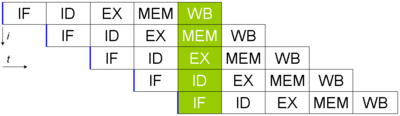
\includegraphics[width=0.45\textwidth]{pipelines}
  \caption{Wikipedia, the free encyclopedia, “Atomic force microscopy,” https://en.wikipedia.org/wiki/File:Fivestagespipeline.png}
  \Description{Stages for instruction queue in common processors}
\end{figure}


\subsection{Avoid Decision statements}

Conditional statements like 'if....else...' translate in assembly to a set of JMP instructions. The JMP instructions require a few additional steps like storing the current Program Counter and updating the Stack Pointer so that the program can resume graceful execution when the control returns to the point from where the JMP was called. These additional steps cost CPU cycles and when possible should be avoided. Several hacks are available to counter these through Arithmetic and Logical operations to obtain results similar to what the conditional statements do. 
In case it is impossible to remove the conditional statements, there should at least be an effort to move the condition statements out of a loop construct so that the overheads related to JMP instruction are not repeated several times. 

Example:
\begin{verbatim}
    int maximum(int a, int b) {
        if (a > b)
            return a;
        else
            return b;
    }
\end{verbatim}
Can be replaced by:
\begin{verbatim}
    int maximum(int a, int b) {
        return -(((b - a) >> 31)*a + ((a - b) >> 31)*b);
    }
\end{verbatim}

Several modern compilers are now capable of replacing such conditional statements with logical and arithmetic instructions.

\subsection{Precompute Constants and Constant Expressions}

Sometimes, code can contain variables that for certain use-cases are not subject to change. Such variables should be eliminated and replaced with constants and constant expressions. For the purpose of clarity, such constants can be implemented using Macros which are computed during compilation. 

\subsection{Procedure Inlining}
Similar to Conditional instructions, procedure calls involves several intermediate steps like storing the program counter, updating the stack pointer and then calling a JMP instruction to the procedure being called and a similar set of steps while returning to the caller. This can be avoided with procedure inlining. Procedure inlining provides an elegant way of structuring the code in a modular fashion while not losing the performance gain by executing the instructions in sequence without the overhead of function call. This is generally accomplished by either a prefix for the procedure definition or an annotation placed before the procedure depending on the type of higher-level language used. 

\subsection{Loop Unrolling}
Loops are often the most compute-intensive sections of the code. Pipeline stalls in loops can be hazardous for the performance of programs since the delay is multiplied by the number of iterations. Hence avoiding pipeline stalls in loops is extremely critical. Loop unrolling is done in three steps:
\begin{enumerate}
\item{Preload registers that are used in computation}
\item{Precompute one sample before the loop begins}
\item{Align compute of older samples with loading of new samples to avoid pipeline stalls}
\end{enumerate}
The method best illustrated in the program below. Note that though this technique optimizes the loop, it is based on the assumption that the processor has enough registers available at this point to be utilized in the loop.

\begin{verbatim}
    Loop :
        load R1,(R6)
        load R2,(R6+1)
        mac R1,R2,R3      //..2 t i c k s
        store R3,(R9)
        add R6,2
        inc R7
    EndLoop
\end{verbatim}

The unrolled version is as below:

\begin{verbatim}
    load R1, (R6)
    load R2, (R6+1)
    add R6, 2
    Loop:  
        load R4, (R6)
        mac R1, R2, R3 ..2ticks
        load R5, (R6+1)
    
        add R6, 2
        store R3, (R9)
    
        load R1,(R6)
        mac R4, R5, R7
        load R2, (R6+1)
    
        add R6, 2
        store R7, (R9)
        inc R9
    Endloop
\end{verbatim}


\subsection{Utilize Special Architecture Capabilities}
Some processors also come with specialized hardware in the form of co-processors, special Multiply-Accumulate units, fast I/O units and others. The compilers may not fully utilize these special facilities provided for the processor. Such handling requires customization of the compilers or disabling compiler optimization and manually modifying sections of code to utilize the capabilities better. For example, most multimedia SOCs provide an additional DSP or a Co-Processor for specialized computation and they can do computations independent of the registers and ALU of the main processors. The compiler may not take advantage of such feature while optimizing and hence require manual intervention by specialist programmers.

In such scenarios, the specialists have advanced knowledge of the Instruction architecture of the processor and the special-purpose processors. They decide on which part of the code shall be executed on the processor and which part would be redirected towards special purpose processors. The special purpose processors could be Signal processors, controllers or just a coprocessor with additional MAC units to enable parallel processing. The programmer can use a switch like \#pragma to separate code that should run on the special purpose processor. In such optimizations, each main processor instruction is coupled with one co-processor instruction that is independent of the main processor instruction and are executed in parallel. 


\section{Superoptimization}

The concept of superoptimization 


\subsection{Understanding Superoptimization}

\subsubsection{The Method}

\subsubsection{Limitations}

\subsubsection{Applications}

\subsection{Peephole Superoptimizers}


\section{Superoptimizers in Modern Compilers}

\section{Other Related Works and Future Direction}


\section{Conclusions}

\bibliographystyle{ACM-Reference-Format}
\bibliography{acmart.bib}

\end{document}